\section{Evaluation} \label{sec:evaluation} 

\subsection{The goal and quality of sequencing process} 

The final goal of sequencing process is to find out the potential matching
coordinates, the number of potential error corresponding to each potential
matching coordinates and the detail information of the difference between input
fragment and subsequences of that coordinates. The potential matching
coordinates are starting coordinates of subsequences whose edit-distance from
the corresponding fragment is under the saturation value (maximum edit
distance), which is decided by the user. The detail information of the
difference involves the type of differences (one of insertion, deletion and
mismatch), the location of each differences and the sort of base pair
corresponding to the location of difference. Figure~\ref{fig:detail_error}
shows the example of the detail difference information. The quality of
sequencing has two factors, time and comprehensiveness. The matching time means
how long does it takes to perform and the comprehensiveness means that how many
coordinate can be determined by matching process. It also can be explained at
the concept of coverage, like how many portion of potential matching points can
be found by the matching process.\\

%%%%%%%%%%%%%%%%%%%%%%%%%%%%%%%%%%%%%%%%%%%%%%%%%%%%%%%%%%%%%%%%%%%%%%%%%%%%%%%%
\begin{figure}[t] \centering
\vspace{0.1in}
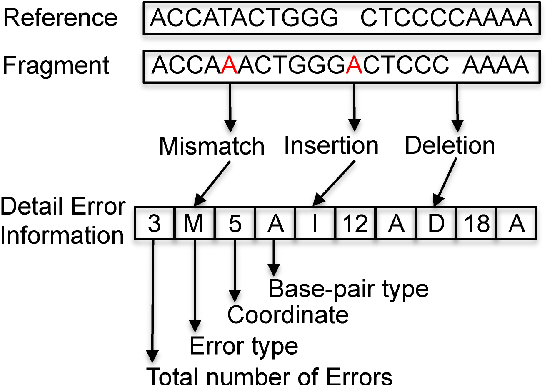
\includegraphics[height=1.8in]{./figure/Detail_Error_B.pdf} \vspace{0in}
\caption{The data structure of detail error}
\label{fig:detail_error} \end{figure}
%%%%%%%%%%%%%%%%%%%%%%%%%%%%%%%%%%%%%%%%%%%%%%%%%%%%%%%%%%%%%%%%%%%%%%%%%%%%%%%%

\subsection{CPU evaluation and Result} 
%%%%%%%%%%%%%%%%%%%%%%%%%%%%%%%%%%%%%%%%%%%%%%%%%%%%%%%%%%%%%%%%%%%%%%%%%%%%%%%%
\begin{figure}[b] \centering
\vspace{0.1in}
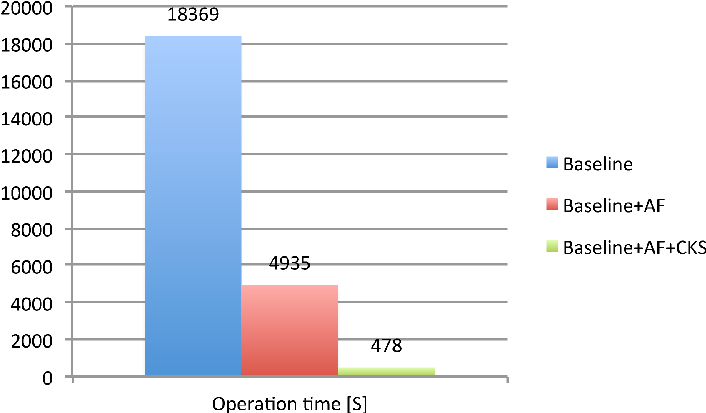
\includegraphics[height=1.8in]{./figure/CPU_Result_B.pdf} \vspace{0in}
\caption{The total sequencing time of CPU implementations}
\label{fig:cpu_result} \end{figure}
%%%%%%%%%%%%%%%%%%%%%%%%%%%%%%%%%%%%%%%%%%%%%%%%%%%%%%%%%%%%%%%%%%%%%%%%%%%%%%%%

First of all, we have to retrieve the hash table to memory for sequencing the
input fragment set to reference sequence. In section~\ref{sec:method_hash}, we
extract 22 hash tables corresponding to each chromosome from reference
sequence.  The matching sequence for the every input fragments is performed
with one of the hash table first. After finishing the matching sequence using
one hash table, then the next hash table is retrieved to the main memory and
the matching sequence is performed again. The reason why we tried to match all
the input fragments to one hash table first is that the required time for
loading hash table takes long time. So, the duplication of hast table loading
process needs to be prevented to improve performance. There are three
comparison methods of sequencing algorithm. The base line of CPU implementation
is no filtering case and its algorithm is almost equal to the algorithm of
mrFAST. After fetching the fragment, it is divided as several keys whose size
is same with hash table key’s length. If \textit{e} error is allowed, first
\textit{e+1} divided fragment sequences are selected as the keys and it tries
to find out the corresponding coordinate with each key from the hash table. The
subsequence of reference sequence, which is located at the coordinate
corresponding to the key, is retrieved from the reference sequence. These two
sequences are compared with each other by string comparison operation. If the
edit-distance between these two sequences is lower than the maximum allowable
edit-distance, then this location is determined as the potential matching
location and the detail information of difference is informed. In this base
line, there is no filtering method, so the string comparison operation is
performed as many as the summation of all key’s corresponding coordinate size.
Second method uses the Adjacency Filtering. Before taking a string comparison,
the Adjacency Filtering is performed to filter out the obviously not matched
coordinates.  After Adjacency Filtering, the string comparison is performed
only when it is passed the Adjacency Filtering. The third method is similar
with the second method. The only difference is that the cheapest \textit{e+1}
key is selected as the searching keys. Figure~\ref{fig:cpu_result} shows the
result of the three versions of CPU implementation. The case using only the
Adjacency Filtering provides 3.7-fold speed up over the base line. The case
using both of the Adjacency Filtering and Cheap Key Selection provides
38.4-fold speedup.\\

\subsection{GPU evaluation and Result} 

%%%%%%%%%%%%%%%%%%%%%%%%%%%%%%%%%%%%%%%%%%%%%%%%%%%%%%%%%%%%%%%%%%%%%%%%%%%%%%%%
\begin{figure}[t] \centering
\vspace{0.1in}
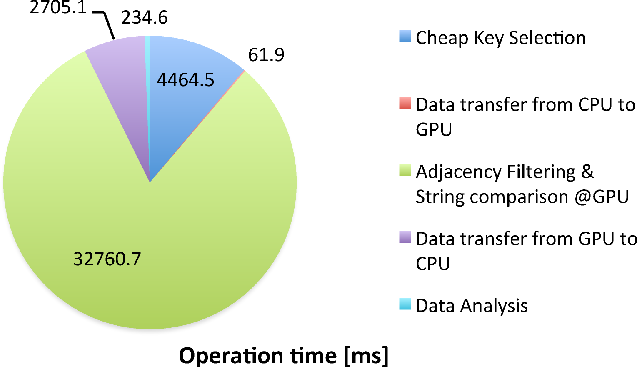
\includegraphics[height=1.8in]{./figure/GPU_portion_B.pdf} \vspace{-0.2in}
\caption{The total sequencing time of CPU implementations}
\label{fig:gpu_portion} 
\end{figure}
%%%%%%%%%%%%%%%%%%%%%%%%%%%%%%%%%%%%%%%%%%%%%%%%%%%%%%%%%%%%%%%%%%%%%%%%%%%%%%%%
%%%%%%%%%%%%%%%%%%%%%%%%%%%%%%%%%%%%%%%%%%%%%%%%%%%%%%%%%%%%%%%%%%%%%%%%%%%%%%%%
\begin{figure}[b] \centering
\vspace{0.15in}
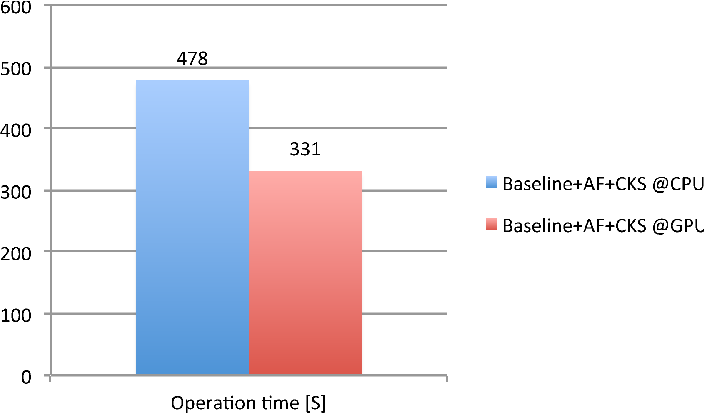
\includegraphics[height=1.8in]{./figure/GPU_Result_B.pdf} \vspace{0in}
\caption{The total sequencing time of CPU and GPU implementations}
\label{fig:gpu_result} 
\end{figure}
%%%%%%%%%%%%%%%%%%%%%%%%%%%%%%%%%%%%%%%%%%%%%%%%%%%%%%%%%%%%%%%%%%%%%%%%%%%%%%%%

Figure~\ref{fig:gpu_portion} shows the time consumptions corresponding to each stage of
sequencing. In the stage of Cheap Key Selection, the input fragment (108
base-pairs length) is divided to 9ea 12 base-pairs length keys and sorted these
keys based on the number of coordinates corresponding to the keys. It takes
about 11\% of total sequencing time. In the stage of input data transfer, the
sorted fragments are shipped to the GPU. After that, GPU operated Adjacency
Filtering and string comparison and it takes about 81.4\% of total sequencing
time. The output data transfer time is about 6.7\% of total sequencing time. The
reason why output data transfer time is quite larger than the input transfer
time, is that output data involves the potential locations, the number of
edit-distance and the detailed information of difference between fragments and
reference.\\

\subsection{FastHASH vs. BWA}

We compared the total sequencing time of FastHASH and BWA in
Figure~\ref{fig:bwa}. The operation option for BWA is -R 10000 -n 3 -N, which
means that the maximum allowable edit-distance is 3 and find out all possible
location within these errors, which is the same condition of FastHASH. Two
tools also used the same input fragment set which has 1 million fragments. For
the sequencing speed, FastHASH is 5.5-fold faster than BWA. For the
comprehensiveness, we compared the number of possible locations which are found
by each tools. FastHASH's result size is about 21 million and BWA's result size
is about 1 million. This means that FastHASH provides quite better
comprehensiveness than BWA. We remain more detail comparison to measure the
comprehensiveness as future work. \\

%%%%%%%%%%%%%%%%%%%%%%%%%%%%%%%%%%%%%%%%%%%%%%%%%%%%%%%%%%%%%%%%%%%%%%%%%%%%%%%%
\begin{figure}[b] \centering 
\vspace{0.15in}
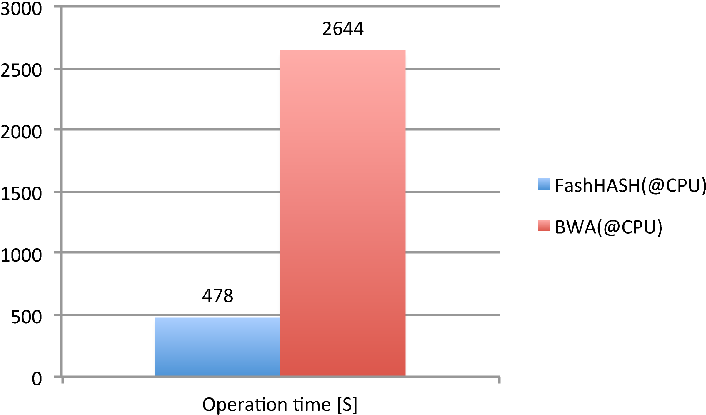
\includegraphics[height=1.8in]{./figure/BWA_B.pdf} \vspace{0in} \caption{The
total sequencing time of FastHASH and BWA} 
\label{fig:bwa} 
\end{figure}
%%%%%%%%%%%%%%%%%%%%%%%%%%%%%%%%%%%%%%%%%%%%%%%%%%%%%%%%%%%%%%%%%%%%%%%%%%%%%%%%
